\documentclass[a4paper,10pt]{article}
\usepackage[utf8]{inputenc}
\usepackage{amsmath}
\usepackage{amsfonts}
\usepackage{amssymb}
\usepackage{graphicx}

\numberwithin{equation}{section}
\renewcommand\thesubsection{\alph{subsection}}
\newcommand{\bvp}[1]{\textbf{#1}'}
\newcommand{\bv}[1]{\textbf{#1}}

%opening
\title{Statistical Mechanics I HW1}
\author{Vince Baker}

\begin{document}

\maketitle

\section{Problem 1}
a) We use the differental relations for T and P:
\begin{gather}
 T=\frac{3As^2}{v}=\frac{\partial u}{\partial s}\\
 P=\frac{As^3}{v^2}=\frac{\partial u}{\partial v}
\end{gather}
From these relations we find:
\begin{gather}
 u(s) = \frac{As^3}{v}+f(v)\\
 u(v) = \frac{As^3}{v}+f(s)
\end{gather}
\\
b) Integrating directly from the differential form:
\begin{gather}
 du = Tds - Pdv = \frac{3As^2}{v}ds - \frac{As^3}{v^2}dv\\
 u = \frac{2As^3}{v}
\end{gather}


\section{Problem 2}
a) Plotting the entropy as a function of $\frac{E_A}{E_A+E_B}$: \\

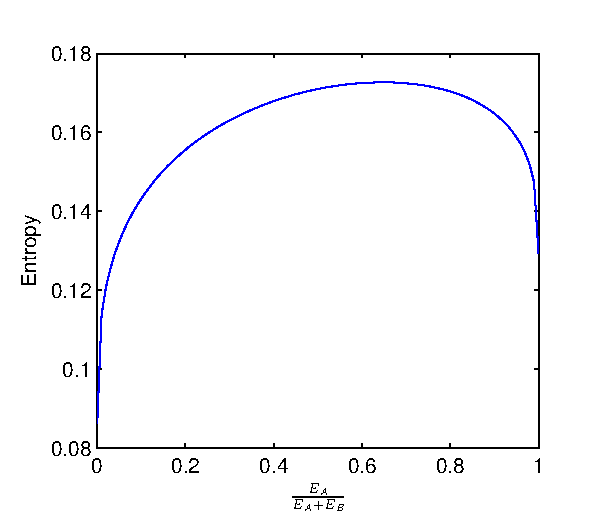
\includegraphics{p1}
\\
We note that the maximum entropy occurs at 0.65.
\\ \\
b) At thermal equillibrium the temperature (and therefore the inverse of the temperature) will be equal.
\begin{gather}
 \frac{1}{T}=\frac{dS}{dE}=\frac{1}{3}(NVE)^{\frac{-2}{3}}NV\\
 \left (\frac{N_BV_BE_B}{N_AV_AE_A}\right )^{\frac{2}{3}}=\frac{N_BV_B}{N_AV_A}\\
 \frac{E_B}{E_A}=\sqrt{\frac{N_BV_B}{N_AV_A}}
\end{gather}
Plugging in the values for $N_A, V_A,N_B,V_B$ we find that $\frac{E_B}{E_A}=0.544$.
\\ \\
c) This is equivalent to $\frac{E_A}{E_A+E_B}=0.65$, 
showing that setting the temperatures equal in the two separate compartments maximizes the total entropy.

\section{Problem 3}
Both gasses start at the same temperature. Using the ideal gas relation to find the pressures:
\begin{gather}
 P_1=\frac{nkT}{nV_0}=\frac{kT}{V_0}\\
 P_2=\frac{mkT}{mV_0}=\frac{kT}{V_0}=P_1
\end{gather}
So both gasses are at the same temperature and pressure to begin.
Therefore, there will be no change in the energies of the components when the partition is ruptured.
We use the entropy relation for ideal gas:
\begin{gather}
 S=NS_0+NRln\left (\left(\frac{U}{U_0}\right )^C\frac{V}{V_0}\right )
\end{gather}
Setting our initial entropies to 0, the total increase is:
\begin{gather}
 S_{H2}=nR\ln{\left(\frac{(n+m)V_0}{nV_0} \right)}\\
 S_{He}=mR\ln{\left(\frac{(n+m)V_0}{mV_0} \right)}\\
 S_{total} = (n+m)R\ln{\left((n+m)V_0\right )}-nR\ln{(nV_0)}-mR\ln{(mV_0)}
\end{gather}


\section{Problem 4}
Starting with the given relations,
\begin{gather}
 e = \frac{3}{2}Pv\\
 P = AvT^4
\end{gather}
To find the Helmholtz potential $F(v,T)=e-Ts$ we need $e(v,T)$ and $s(v,T)$. 
\begin{gather}
 e = \frac{3}{2}Pv\\
 e(v,T) = \frac{3}{2}Av^2T^4
\end{gather}
To find $s(v,T)$ we integrate the relation $T=\frac{\partial e}{\partial s}$.
\begin{gather}
 T=\frac{de}{ds}\\
 ds = \frac{1}{T}de\\
 s = \int 6Av^2T^2 dT\\
 s(v,T) = 2Av^2T^3
\end{gather}
The Helmholtz potential is then $f=u-Ts=-\frac{1}{2}Av^2T^4$.\\ \\
To find the Gibbs potential $g(P,T)=f-Pv$ we need $v(P,T)=\frac{P}{AT^4}$ and
$f(P,T)$.
\begin{gather}
 f=-\frac{1}{2}Av^2T^4=-\frac{1}{2}AT^4\left(\frac{P}{AT^4}\right)^2\\
 f(P,T) = -\frac{1}{2}\frac{P^2}{AT^4}
\end{gather}
We can then find $G(P,T) = f-Pv = -\frac{3}{2}\frac{P^2}{AT^4}$. 


\section{Problem 5}
a) We show that S is an extensive parameter through direct scaling.
\begin{gather}
 S(V,E)=\frac{4}{3}\sigma V^{\frac{1}{4}}E^{\frac{3}{4}}\\
 S(\lambda V, \lambda E) = (\lambda)^{\frac{1}{4}}(\lambda)^{\frac{3}{4}}
 \frac{4}{3}\sigma V^{\frac{1}{4}}E^{\frac{3}{4}}\\
  S(\lambda V, \lambda E) = \lambda S(V,E)
\end{gather}
\\ 
b) We find the temperature from the differential definition.
\begin{gather}
 \frac{1}{T}=\left (\frac{\partial S}{\partial E} \right )_V=
    \sigma\left ( \frac{V}{E} \right )^{\frac{1}{4}}\\
 T = \frac{1}{\sigma} \left(\frac{E}{V} \right)^{\frac{1}{4}}
\end{gather}
To find the pressure, we rearrage (5.1) to find $E(S,V)$ and use $P=-\frac{\partial E}{\partial V}$.
\begin{gather}
 E(V,S) = \left(\frac{(\frac{3S}{4\sigma})^4}{V} \right)^{\frac{1}{3}}\\
 -\frac{\partial E}{\partial V}=-\frac{1}{3}\left(\frac{(\frac{3S}{4\sigma})^4}{V} \right)^{-\frac{2}{3}}
 \left(-\frac{(\frac{3S}{4\sigma})^4}{V^2} \right)\\
 P=\frac{1}{3}\left(\frac{3S}{4\sigma V} \right)^{\frac{4}{3}}
\end{gather}
\\
c) Starting with the Euler relation, and inserting the equation for T found above:
\begin{gather}
 TS-PV=E\\
 \frac{1}{\sigma} \left(\frac{E}{V} \right)^{\frac{1}{4}} \times \frac{4}{3}\sigma V^{\frac{1}{4}}E^{\frac{3}{4}}
 -PV = E\\
 PV = \frac{1}{3}E
\end{gather}

\end{document}
